\section{Progettazione di un sistema di ML}

La progettazione di un sitema di \emph{machine learning} può essere sintetizzata nelle seguenti fasi:
\begin{enumerate}
\item analisi e \emph{pre-processing} dei dati;
\item \emph{feature} selection;
\item scelta del modello ed addestramento;
\item validazione del modello sul \emph{validation set} ed eventualmente si ritorna al passo precedente;
\item valutazione delle prestazioni su un \emph{test set};
\item adozione del modello nel contesto finale.
\end{enumerate}
Analizziamo di seguito le singole fasi.

\subsection{Analisi e pre-processing dei dati}
\subsubsection{Pulizia dei dati}
I dati ricevuti e provenienti dal mondo reale potrebbero essere sporchi, ovvero:
\begin{itemize}
\item potrebbero essere incompleti, ad esempio alcuni valori di un attributo sono mancanti;
\item potrebbero essere inaccurati o discostarsi molto da quanto ci si aspetterebbe (ad esempio a causa di una digitazione errata da parte di un operatore umano).
\end{itemize}
Poiché vale la regola GIGO (Garbage In - Garbage Out) secondo cui un modello addestrato con dati sporchi produrrà risultati non affidabili, è necessario individuare tutte queste anomalie e ripulire i dati. Per quanto questa operazione non segua sempre un flusso standard, ma dipende dai particolari dati e dalle proprietà che possiamo osservare, si possono distinguere alcune operazioni comuni:
\begin{itemize}
\item rimozione degli \emph{outlier}: per \emph{outlier} si intendono gli esempi il cui valore d'uscita supera il terzo quartile (\autoref{sec:quantili});
\item rimozione dei duplicati: un campione d'addestramento duplicato non aggiunge alcune informazione utile;
\item rimozione del rumore: cioè delle informazioni inutili (ad esempio l'ID utente è tipicamente un valore non significativo ai fini della classificazione).
\end{itemize}

\paragraph{Quantili e quartili}\label{sec:quantili}
L'$\alpha$-quantile, con $\alpha \in [0,1]$, identifica quel valore $x_\alpha$ tale che una quota $\alpha$ della popolazione delle $x$ sia $\leq x_\alpha$.
Esistono diversi quantili tipicamente utilizzati, e sono:
\begin{itemize}
\item quartili, dividono la distribuzione in 4 parti uguali. Ciascun quartile rappresenta il 25\% della popolazione (quindi il terzo quartile è quel valore di $x$ di cui il 75\% della popolazione è più piccolo);
\item decili, dividono la popolazione in 10 parti uguali (ciascun decile rappresenta il 10\% della popolazione);
\item percentili, dividono la popolazione in 100 parti uguali (ciascuna parte rappresenta l'1\% della popolazione).
\end{itemize}

\subsubsection{Pre-processing}
Oltre ad aver pulito i dati è necessario pre-elaborarli prima di darli in pasto al classificatore, alcune operazioni comuni sono:
\begin{itemize}
\item discretizzazione ed aggregazione, ad esempio potremmo raggruppare gli ingressi in base all'attributo ``età'' in ``adulti'', ``ragazzi'' e ``bambini'';
\item normalizzazione e \emph{re-scaling} (trattate nel paragrafo successivo);
\item creazione di nuovi attributi, ad esempio quando adottiamo un GLM stiamo aumentando il numero di feature. Ciò è utile a patto che consenta una separazione più netta delle classi, se ciò non accade introduciamo una complicazione superfla al problema.
\end{itemize}

\paragraph{Normalizzazione e re-scaling}\label{feature_scaling}
La normalizzazione consiste nel restringere l'intervallo di variabilità di un attributo preservando le distanze relative tra i suoi valori. Il \emph{re-scaling} è un semplice cambio di scala, cioè divisione o moltiplicazione per uno stesso valore.

Queste operazioni si rendono necessarie perché ciascun attributo può variare in un intervallo più o meno ampio rispetto agli altri (ad esempio l'altezza ed il peso espressi in cm e kg hanno intervalli di variabilità molto diversi). Molti algoritmi di classificazione non riescono ad operare su dati così fatti, ad esempio la funzione logistica satura ad 1 quando l'ingresso è troppo grande. Anche lì dove questo problema non si presenta, come nella regressione lineare, si vede che l'algoritmo di discesa a gradiente converge più velocemente quando i dati sono normalizzati\footnote{\href{http://www.youtube.com/watch?v=PINX6Mk636M}{Coursera, Machine Learning (Andrew Ng), Lezione 4.3} }. Ribadiamo ulteriormente  che ciascun attributo viene normalizzato separatamente dagli altri e lo scopo della normalizzazione è far sì che tutti gli attributi varino in uno stesso intervallo. Una volta normalizzati gli ingressi, occorre memorizzare i parametri usati per la normalizzazione, in maniera tale che questa possa essere riapplicata invariata agli ingressi incontrati in fase di predizione. Le tecniche principali sono:
\begin{itemize}
\item \emph{min-max normalization}, si scalano i valori dell'attributo in funzione del minimo e del massimo per farli rientrare in un intervallo [a,b] desiderato (tipicamente [0,1]).
\begin{equation*}
x_i \leftarrow \frac{x_i - \min_i(x_i)}{\max_i(x_i) - \min_i(x_i)} \cdot (b-a) +a
\end{equation*}

\emph{Svantaggi:} 
\begin{enumerate}
\item gli \emph{outlier} influiscono molto su min e max, e quindi sulla normalizzazione;
\item in fase di predizione potrebbe arrivare un ingresso al di fuori dell'intervallo $[\min, \max]$ per cui la normalizzazione sarebbe errata (in risultato sarebbe più piccolo di $a$ o più grande di $b$).
\end{enumerate}
\item \emph{z-score normalization}, normalizza i valori nell'intervallo [-1,1] e si basa su valor medio e deviazione standard, quindi non subisce l'influenza degli \emph{outlier}.
\begin{equation*}
x_i \leftarrow \frac{x_i - \overline{x}}{\sigma_{x}}
\end{equation*}

\end{itemize}

\subsection{Feature selection}
Possono capitare spesso due scenari:
\begin{itemize}
\item nel \emph{dataset} sono presenti attributi superflui. Ad esempio in una base di dati che contiene $\langle$ID, altezza, peso, sesso$\rangle$, l'ID è superfluo ai fini della classificazione;
\item alcuni attributi sono linearmente dipendenti e quindi mantenerne uno solo è sufficiente, dato che tutti gli altri non aggiungi informazione. Ad esempio se il \emph{dataset} prevede $\langle$sesso, peso (kg), peso (lb)$\rangle$ è evidente che uno dei due pesi è eliminabile.
\end{itemize}

Ridurre le dimensioni dei vettori delle \emph{feature} consente di semplificare il problema e ciò si traduce in tempi di addestramento più brevi e modelli meno complessi (di grado inferiore, riducendo dunque il rischio di \emph{overfitting}).

Le tecniche adottate per individuare gli attributi superflui sono:
\begin{enumerate}
\item Filtri: grazie ai quali è possibile stabilire un \emph{ranking} degli attributi in cui gli ultimi sono quelli che discriminano meno la classe di appartenenza dell'esempio (misure tipiche: \emph{information gain}, \emph{entropy}, \emph{mutual information});
\item \emph{Wrappers:} si suddivide il \emph{set} di dati di addestramento in due parti. La prima parte viene utilizzata per addestrare il modello, selezionando però solo un sottoinsieme di attributi per volta. Per ciasucno di questi sottoinsiemi si valutano le prestazioni sulla seconda parte (\emph{validation set}) per capire quali attributi hanno influenza maggiore;
\item Algoritmi di riduzione della dimensionalità (PCA, trattata in seguito).
\end{enumerate}

\subsection{Scelta del modello}\label{sec:overunderfitting}
\subsubsection{Overfitting ed underfitting}
Nella scelta del modello è importante evitare due situazioni:
\begin{itemize}
\item \emph{overfitting}: si verifica quando il modello si comporta molto bene sul \emph{training set} ma non è in grado di prevedere correttamente le classi dei campioni nel \emph{validation set}. Significa che il modello non è in grado di generalizzare ed è quindi troppo complesso (grado troppo elevato). Un modello troppo complesso oscillerà molto e sarà caratterizzato da una forte varianza.
\item \emph{underfitting}: il modello è troppo semplice e genera errori troppo grandi sia sui dati di addestramento che su quelli di validazione. Ciò si traduce in un errore medio di predizione elevato (\emph{bias});
\end{itemize}

\subsubsection{Trade-off tra bias e varianza}
Cerchiamo di capire qual è l'influenza di \emph{bias} e varianza sull'errore mediamente commesso da un modello\footnote{Questa parte è stata scritta partendo dagli appunti ed integrandoli con il libro e con quanto letto \href{http://www-scf.usc.edu/~csci567/17-18-bias-variance.pdf}{qui}.}.

\paragraph{Formulazione del problema}
Ipotizziamo di avere a disposizione infiniti \emph{dataset} $D_i$ la cui unione costuituisce l'intera popolazione di campioni che il nostro modello potrà mai incontrare nella sua esistenza.

Ipotizziamo di fissare il tipo di modello da usare (ad esempio il grado del polinomio di una regressione lineare) e di addestrarlo ogni volta con un diverso $D_i$, otterremo quindi infinite ipotesi $h^{(D_i)}(x)$.

Ciascun campione del \emph{dataset} è nella forma $<\mathbf{x^{(i)}}, y^{(i)}>$ dove $y^{(i)}$ è somma di un valore vero (a noi sconosciuto) e di un errore gaussiano a media nulla e varianza $\sigma_e$:
\begin{equation*}
y^{(i)}=f(\mathbf{x^{(i)}})+e^{(i)}
\end{equation*}


Ciascuna delle ipotesi $h^{(D_i)}$ commetterà un errore nel predire i campioni \emph{rispetto al loro valore vero}, e lo possiamo esprimere sotto forma di errore quadratico medio (MSE):
\begin{equation*}
MSE\left(h^{(D_i)}(x)\right) =E_x\left[(h^{(D_i)}(x)-f(x))^2\right]
\end{equation*}

A noi interessa valutare l'aspettazione (valore atteso) di quest'ultima quantità rispetto ai $D_i$. In pratica è come se misurassimo l'errore quadratico  medio  commesso da ciascun singolo modello su tutti i possibili ingressi e mediassimo a loro volta questi risultati; ovviamente il calcolo di questo valor medio richiederebbe la conoscenza di tutti gli infiniti $D_i$, per cui ci accontentiamo del valore atteso (che chiameremo \emph{Generalization Error} o \emph{GER}):
\begin{dmath*}
GER = E_D[MSE] = E_D\left[E_x\left[\left(h^{(D_i)}(x)-f(x)\right)^2\right]\right] 
= E_x\left[E_D\left[\left(h^{(D)}(x^{(i)})-f(x^{(i)})\right)^2\right]\right]
\end{dmath*}

L'ultimo passaggio è possibile perché l'operatore $E$ è lineare (si tratta di una sommatoria nel caso discreto). Essendo tutti gli addendi di $E_x$ non negativi, per ottenere un \emph{GER} piccolo non ci resta che minimizzare $E_D$. La presenza degli apici  $(i)$ nella formula più interna, ci ricorda che l'aspettazione $E_D$ che desideriamo conoscere è calcolata fissato un singolo campione $x^{(i)}$ e facendo variare il modello usato.

\paragraph{Decomposizione}
Studiamo ora come è fatto il termine\footnote{La decomposizione del MSE in \emph{bias} e varianza è valida in generale. Qui riportiamo la dimostrazione usando la notazione del contesto in analisi.}:

\begin{equation}\label{eq-aspettazione}
E_D\left[\left(h^{(D)}(x^{(i)})-f(x^{(i)})\right)^2\right].
\end{equation}
Introduciamo la grandezza:
\begin{equation*}
\overline{h}(x^{(i)}) = E_D\left[h^{(D)}(x^{(i)})\right]
\end{equation*}
che rappresenta la media statistica dei valori restituiti in uscita da ciascun modello $h^{(D_i)}$ quando tutti ricevono in ingresso uno stesso $x^{(i)}$. In altre parole fissiamo $x^{(i)}$, lo diamo in pasto a tutti i modelli addestrati e calcoliamo la media delle uscite. Questa quantità rappresenterà la miglior stima di $f(x^{(i)})$.

A questo punto sommiamo e sottraiamo $\overline{h}(x^{(i)})$ nell'\autoref{eq-aspettazione}:

\begin{dmath*}
E_D\left[\left(h^{(D)}(x^{(i)})-\overline{h}(x^{(i)})+\overline{h}(x^{(i)})-f(x^{(i)})\right)^2\right]
\end{dmath*}
sviluppiamo il quadrato raggruppando gli addendi 2 per volta e sfruttiamo la linearità di $E$:
\begin{dmath*}
E_D\left[\left(h^{(D)}(x^{(i)})-\overline{h}(x^{(i)})\right)^2\right] +E_D\left[\left(\overline{h}(x^{(i)})-f(x^{(i)})\right)^2 \right]+ E_D\left[2\left( h^{(D)}(x^{(i)})-\overline{h}(x^{(i)})\right) \left( \overline{h}(x^{(i)})-f(x^{(i)})\right)\right]
\end{dmath*}
Analizziamo ora i singoli addendi. Il primo rappresenta, per definizione, la varianza:
\begin{equation*}
E_D\left[\left(h^{(D)}(x^{(i)})-\overline{h}(x^{(i)})\right)^2\right] = Var\left(h^{(D)}(x^{(i)})\right).
\end{equation*}
Nel secondo termine entrambi gli addendi non dipendono più da $D$, fissato un $x^{(i)}$ rappresentano dei numeri, per cui:
\begin{equation*}E_D\left[\left(\overline{h}(x^{(i)})-f(x^{(i)})\right)^2 \right]= (\overline{h}(x^{(i)})-f(x^{(i)}))^2
\end{equation*}
e questa quantità rappresenta per definizione il $Bias^2\left(h^{(D)}(x^{(i)})\right)$. Lo stesso discorso può essere fatto per il terzo fattore del terzo addendo:
\begin{dmath*}
2\left( \overline{h}(x^{(i)})-f(x^{(i)})\right)\left E_D[h^{(D)}(x^{(i)})-\overline{h}(x^{(i)}) \right] 
=2\left( \overline{h}(x^{(i)})-f(x^{(i)})\right) \left( E_D\left[ h^{(D)}(x^{(i)})\right]-E_D\left[\overline{h}(x^{(i)}) \right]\right)
=2\left( \overline{h}(x^{(i)})-f(x^{(i)})\right) \left(\overline{h}(x^{(i)})-\overline{h}(x^{(i)})\right)=0
\end{dmath*}

In definitiva:

\begin{dmath*}
MSE(h^{(D)}(x^{(i)})) 
= Bias^2\left(h^{(D)}(x^{(i)})\right) + Var\left(h^{(D)}(x^{(i)})\right).
\end{dmath*}

\paragraph{Commento dei risultati}
L'errore di generalizzazione di un modello è l'aspettazione del MSE appena definito, abbiamo quindi interesse a rendere l'MSE piccolo. Ciò può essere ottenuto riducendo il \emph{bias} o la varianza:
\begin{itemize}
\item il \emph{bias} tiene conto di quanto la migliore stima (cioè la media delle stime) sia in grado di avvicinarsi al valore vero. Un \emph{bias} alto è indice di un modello troppo semplice che, a prescindere dal \emph{dataset} $D_i$ di addestramento, non ha una buona capacità predittiva. Questo è riconducibile ad un polinomio di grado troppo basso;
\item la varianza tiene conto di quanto ciascuna ipotesi si discosta dal valor medio calcolato su tutte le ipotesi. Una varianza alta è indice del fatto che, addestrando uno stesso modello con $D_i$ diversi, si possono ottenere ipotesi molto diverse. Ciò significa che il modello è troppo complesso, tende ad andare in \emph{overfitting} e manca di capacità di generalizzazione.
\end{itemize}


L'ideale sarebbe avere sia \emph{bias} che varianza piccoli, ciò garantisce che il modello approssimi bene i risultati reali pur rimanendo stabile, cioè non subisce fortemente l'influenza del particolare \emph{training set} utilizzato (a patto che questo sia ben costruito). In \autoref{fig:bias_vs_varianza} è mostrato il tipico andamento di \emph{bias} e varianza in funzione della complessità del modello. Notiamo che le due componenti hanno un andamento opposto (al diminuire dell'una, aumenta l'altra), il miglior compromesso è rappresentato dal punto in cui la loro somma è minima.

\begin{figure}[tbp]
\centering
  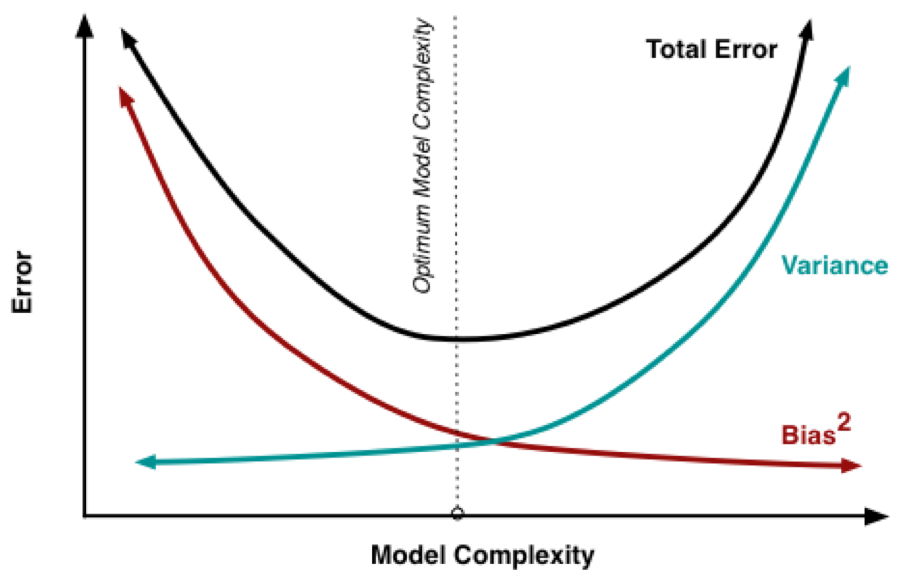
\includegraphics[width=0.6\textwidth]{images/bias_vs_var}
  \caption{\emph{Bias} e varianza in funzione della complessità del modello.}
  \label{fig:bias_vs_varianza}
\end{figure}


\subsubsection{Cross-validation}

Non sapendo quale modello scegliere, l'idea della \emph{cross-validation} è quella di addestrarne alcuni su un sottoinsieme del \emph{training set} a disposizione e poi valutarne le prestazioni sulla restante parte (\emph{validation set}).

La scelta del modello finale va fatta sulla base delle misure di prestazione calcolate sul \emph{validation set} e non sul \emph{training set}. Questo ha senso perché il modello è stato addestrato per minimizzare l'errore quadratico sul \emph{training set} ed in virtù di  ciò ci aspettiamo che l'errore commesso su di esso sia basso. In particolare, si dimostra che l'errore commesso su \emph{training set} è una sottostima dell'errore di generalizzazione, mentre quello sul \emph{validation set} lo approssima in maniera migliore.

Dopo aver scelto quale modello usare, questo può essere riaddestrato utilizzando tutto il \emph{training set} iniziale.

Questo stesso approccio può essere sfruttato per determinare metaparametri (ad esempio il coefficiente di penalizzazione del fattore di regolarizzazione) oppure per capire quali siano le \emph{feature} meno significative.

Due tecniche comunemente usate per effettuare \emph{cross-validation} prendono il nome di \emph{holdout} e \emph{k-folds}

\begin{figure}[]
\centering
  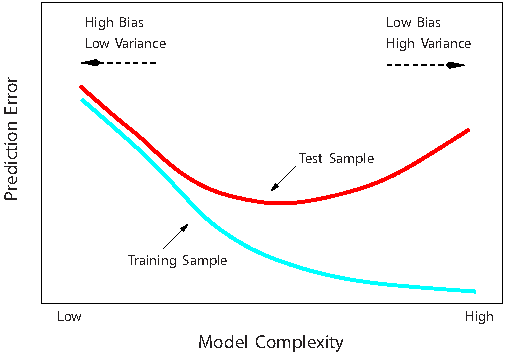
\includegraphics{images/bias_varianza}
  \caption{Errore di predizione su \emph{trainig set} e \emph{validation set} al variare della complessità del modello}
  \label{fig:bias_varianza}
\end{figure}

\subsubsection{Holdout cross validation}
La \emph{holdout cross validation} prevede che il \emph{training set } su cui addestrare i modelli in prova sia costituito dai due terzi di quello iniziale, il restante terzo costituirà il \emph{validation set}. Occorre prestare attenzione affinché i campioni scelti per l'addestramento e per la valutazione siano rappresentativi di tutte le classi presenti. Se ad esempio la classe 0 è completamente assente tra i dati di addestramento, e presente in quelli di validazione, il modello mostrerà una pessima capacità di riconoscere tali campioni e ciò si ripercuoterà negativamente sulle misure di prestazione.


\subsubsection{K-folds cross validation}
Questa tecnica prevede che l'insieme dei dati venga suddiviso in $k$ sottoinsiemi (tipicamente $k=10$). Durante ciascuna delle $k$ iterazioni dell'algoritmo, ciascun modello viene addestrato sull'unione di $k-1$ sottoinsiemi, e validato sul $k-esimo$. Ad ogni iterazione si cambiano i $k-1$ sottoinsiemi di addestramento e di conseguenza il $k-esimo$. L'errore commesso da ciascun modello viene calcolato come media degli errori da esso commessi in seguito a ciascuno dei $k$ addestramenti.

\subsection{Valutazione del modello}
La valutazione finale del modello viene fatta dopo averlo scelto, e quindi dopo averlo riaddestrato usando l'unione di \emph{training set} e \emph{validation set}. È evidente, quindi, che il \emph{test set} su cui valutiamo le prestazioni del modello debba essere distinto dagli altri due.

Occorre, inoltre, evitare il \emph{peeking}, cioè non usare i dati del \emph{test set} come se fossero parte del \emph{validation set}. In questa maniera il \emph{test set} viene usato per guidare la scelta del modello (è grave quasi come usare il \emph{test set} per l'addestramento), mentre per ottenere misure di prestazione credibili il \emph{test set} non deve avere alcuna influenza su come il modello viene scelto ed addestrato.


\subsubsection{Matrice di confusione e metriche}
La matrice di confusione consente di rappresentare in maniera compatta alcune grandezze di interesse per il calcolo delle misure di prestazione di un classificatore binario. Supponendo che l'uscita del classificatore sia \emph{yes} ($y=1$) o \emph{no} ($y=0$), la matrice di confusione viene costruita indicando sulle righe la classe reale dei campioni del \emph{test set}, sulle colonne la classe predetta dal classificatore per tali campioni (\autoref{fig:confusione}).



All'interno della matrice indichiamo 4 quantità:
\begin{itemize}
\item TP (\emph{true positive}), rappresenta il numero di veri positivi, cioè il numero di campioni classificati come positivi (classe 1) e che effettivamente sono positivi;
\item TN (\emph{true negative}), rappresenta il numero di veri negativi, cioè il numero di campioni classificati come negativi (classe 0) e che effettivamente sono negativi;
\item FP (\emph{false positive}), rappresenta il numero di falsi positivi, cioè il numero di campioni classificati come positivi (classe 1), ma che in realtà sono negativi;
\item FN (\emph{false negative}), rappresenta il numero di falsi negativi, cioè il numero di campioni classificati come negativi (classe 0), ma che in realtà sono positivi.
\end{itemize}
Osserviamo che:
\begin{itemize}
\item TP+TN+FP+FN è il  numero totale di campioni nel \emph{test set};
\item TP+FN è il numero di istanze positive nel \emph{test set};
\item TN+FP è il numero di istanze negative nel \emph{test set};
\item TP+FP è il numero di predizioni positive a partire dal \emph{test set};
\item TN+FN è il numero di predizioni negative a partire dal \emph{test set}.
\end{itemize}
Partendo da queste 4 quantità si definiscono alcune metriche di uso comune:
\begin{itemize}
\item \emph{Accuracy}, rappresenta il tasso di predizioni corrette:
\begin{equation*}
Accuracy = \frac{TP + TN}{TP+TN+FP+FN}
\end{equation*}
\item \emph{Error rate}, rappresenta il tassso di predizioni errate (complemento ad 1 dell'\emph{accuracy}):
\begin{equation*}
Error~Rate = 1 - Accuracy = \frac{FP + FN}{TP+TN+FP+FN}
\end{equation*}
\end{itemize}

\begin{figure}[]
\centering
  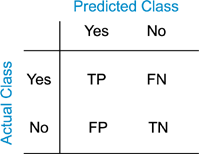
\includegraphics[width=0.3 \textwidth]{images/confusionmatrix}
  \caption{Matrice di confusione}
  \label{fig:confusione}
\end{figure}


Le due metriche precedenti tengono conto delle prestazioni complessive del classificatore. Non ci consentono di capire quanto sia buono nel discriminare casi positivi e casi negativi. A tal proposito vengono adottate le seguenti misure:
\begin{itemize}
\item \emph{Recall}, detta anche \emph{Sensitivity} o \emph{True Positive Rate}, rappresenta la percentuale di casi positivi correttamente calssificati:
\begin{equation*}
Recall = \frac{TP}{TP+FN}
\end{equation*}
\item \emph{Specificity}, detta anche  \emph{True Negative Rate}, in maniera duale alla precedente rappresenta la percentuale di casi negativi correttamente calssificati:
\begin{equation*}
Specificity = \frac{TN}{TN+FP}
\end{equation*}
\item \emph{False Positive Rate}, rappresenta il complemento ad uno della \emph{Specificity}, cioè la percentuale di casi negativi erroneamente classificati:
\begin{equation*}
False~Positive~Rate = 1 - Specificity =  \frac{FP}{TN+FP}
\end{equation*}
\end{itemize}
In ultimo può essere interessante valutare la \emph{Precision}, cioè il tasso di predizioni vere che si rivelano corrette, ovvero il rapporto tra i veri positivi e tutti i positivi:
\begin{equation*}
Precision = \frac{TP}{TP+FP}.
\end{equation*}
Tipicamente vorremmo un classificatore con \emph{Recall} e \emph{Precision} alte, cioè un classificatore con un alto numero di veri positivi e pochi falsi negativi e falsi positivi. Per unire queste due esigenze in un'unica metrica viene introdotta la \emph{F-measure}, calcolata come media armonica di \emph{Precision} e \emph{Recall}:
\begin{equation*}
\text{\emph{F-measure}} = 2\frac{Precision \cdot Recall}{Precision+Recall}.
\end{equation*}


\subsubsection{Curve ROC}

\begin{figure}[tbp]
\centering
  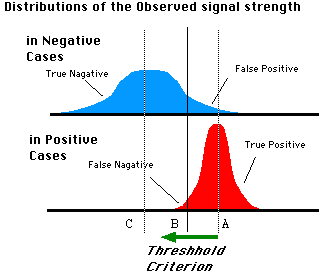
\includegraphics[width=0.5 \textwidth]{images/ROC_distribuzione}
  \caption{Distribuzione delle uscite associate ai campioni positivi e negativi nel \emph{test set}}
  \label{fig:ROC_distribuzione}
\end{figure} 
Vediamo ora come è possibile usare le informazioni provenienti dalle metriche appena introdotte per effettuare il \emph{tuning} di alcuni parametri del modello. 

Ipotizziamo di lavorare con una regressione logistica. Come abbiamo visto in precedenza, l'uscita della funzione ipotesi è numerica ed è compresa tra 0 ed 1. La classe di appartenenza di ciascun campione viene calcolata in base al fatto che tale uscita superi o meno un valore di soglia (\emph{threshold}). In precedenza, però, non abbiamo discusso su come debba essere scelta questa soglia.

Supponiamo che le distribuzioni delle uscite che il classificatore associa ai campioni di classe $1$ e $0$ del \emph{test set} siano gaussiane, rappresentate rispettivamente in azzurro e rosso in \autoref{fig:ROC_distribuzione}.


Se B rappresenta il valore di soglia scelto, è facile vedere che:
\begin{itemize}
\item i campioni negativi a sinistra di B rappresentano i veri negativi;
\item i campioni negativi a destra di B rappresentano i falsi positivi;
\item i campioni positivi a sinistra di B rappresentano i falsi negativi;
\item i campioni positivi a destra di B rappresentano i veri positivi.
\end{itemize}
Quindi la scelta della soglia influisce direttamente sulla matrice di confusione, e quindi sulle metriche analizzate. 

Tramite le curve ROC siamo in grado di vedere esattamente come il valore della soglia influisce sul \emph{True Positive Rate} e sul \emph{False Positive Rate}. Per tracciare una curva ROC facciamo variare la soglia in un intervallo di possibili valori, per ciascun valore calcoliamo \emph{True Positive Rate} e \emph{False Positive Rate} e disegniamo il punto individuato da questa coppia di valori su un sistema di assi cartesiani. La curva risultante rappresenterà l'andamento di \emph{TPR} e \emph{FPR} al variare della soglia (\autoref{fig:ROC}). A seconda di quali sono le esigenze del caso specifico, sceglieremo il valore di soglia più opportuno.

\begin{figure}[tbp]
\centering
  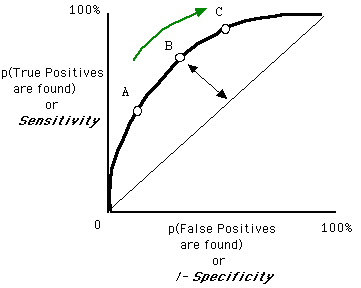
\includegraphics[width=0.5 \textwidth]{images/ROC}
  \caption{Curva ROC}
  \label{fig:ROC}
\end{figure}

Ad esempio, ipotizziamo che il sistema che stiamo addestrando consenta di classificare un paziente come sano o malato. Ovviamente vorremmo che esso fosse in grado di rivelare il 100\% dei malati, ovvero ottenere un \emph{TPR} pari ad 1. Paradossalmente potremmo ottenere ciò impostando una soglia nulla in maniera tale che tutti i pazienti vengano riconosciuti come malati, a prescindere dall'effettivo stato di salute. Da un punto di vista medico questo implicherebbe ulteriori esami sui pazienti per verificare l'effettiva presenza della malattia, e quindi un costo superiore da sostenere (per il paziente o per la Sanità Pubblica). Quindi ciò che vorremmo fare è anche minimizzare il \emph{FPR}, ed ecco che la curva ROC ci consente di individuare il giusto compromesso tra un \emph{TPR} alto ed \emph{FPR} basso. 
Nello stesso scenario, però, potremmo ipotizzare che la malattia sia grave e quindi potrebbe essere preferibile qualche falso positivo in più pur di non abbassare il tasso di veri positivi, evitando quindi che alcuni pazienti malati non vengano riconosciuti come tali. Anche in questo caso l'analisi della curva ROC può farci capire quale sia il miglior valore della soglia.

Le curve ROC possono essere usate anche per determinare i valori ottimali di altri metaparametri del modello, o per fare un confronto tra modelli diversi. In particolare possiamo tracciare la curva ROC di uno stesso modello, addestrato sullo stesso \emph{training set}, modificando di volta in volta il valore un metaparametro. Dopo ciascun addestramento possiamo tracciare la curva ROC e selezionare il modello la cui curva è migliore, cioè quella che sottende l'area maggiore, avvicinandosi maggiormente all'andamento ideale costante di una una retta passante per \emph{TPR}=1. 